\subsection{(Anti-)(hyper-)nuclei production} 
%PHYSICS CASE for anti-hyper-nuclei:
%\begin{itemize}
%\item precision era in anti hyper nuclei observables --> precision test of thermal model and coalescence
%\item solve anti-nuclei puzzle (fragile objects survival in the hadronic phase)
%\item nucleon-nucleon and nucleon-hyperon potential
%\item discovery potential for the A = 4 anti-hyper-nuclei.
%\item impact for astrophysics: EOS of neutron stars 
%\item impact for DM searches
%\item impact on possible new experiments / new lines of research in the next decade
%\end{itemize}
\subsubsection{Thermal production and nucleon coalescence models}
The production of light (hyper-)nuclei and their anti-matter counterparts is modelled within the two scenarios of thermal-statistical hadronisation and coalescence model.
In the thermal-statistical approach \cite{Andronic:2010qu, Andronic:2017}, particles are produced from a fireball in thermal and kinetic equilibrium with temperatures of the order of $T_{chem} \approx$ 156 MeV that are near the temperature of the QCD phase transition boundary, as predicted by lattice QCD calculations \cite{Bazavov:2014pvz,Bellwied:2013cta}.
The yields of the produced objects depend on the chemical freeze-out temperature $T_{chem}$ (when inelastic collisions cease) and the mass of the object $m$, and approximately scale as d$N$/d$y \propto \exp(-m/T_{chem})$.  
Thermal-statistical models have been successful in describing light-flavour particle production across a wide range of energies in nucleus-nucleus collisions \cite{Andronic:2017, Acharya:2017bso}.  
Due to their large mass, light (anti-)(hyper-)nuclei are particularly sensitive to $T_{chem}$ and since they are not affected by feed-down from higher mass states, the measurement of their production constitutes a precision test for the thermal model.  
In the coalescence scenario, composite objects are formed at kinetic freeze-out by coalescence of nucleons that are close in configuration and momentum space \cite{Butler:1963, Kapusta:1980, Bergstrom:1979gpv, Sato:1981ez, Nagle:1996vp, Scheibl:1998tk}. Calculations of the coalescence probability based on a density matrix approach \cite{Scheibl:1998tk} require the knowledge of the nucleus wave-function and identify the volume of the particle source with the homogeneity volume that can be extracted via HBT interferometry \cite{Wiedemann:1999qn}. 
The quantum-mechanical nature of the process is encoded in an average quantum-mechanical correction factor that depends on the size of the nucleus, on the homogeneity volume of the particle source and, via the latter, on the transverse momentum of the coalescing nucleons.

While there are several theory groups working on the calculation of the expected coalescence \cite{Scheibl:1998tk, Cho:2017dcy, Zhang:2018euf, Bazak:2018hgl, Zhao:2018lyf} and thermal production rates \cite{Andronic:2010qu, Wheaton:2004qb, Petran:2013dva}, predictions reported in Fig. \ref{fig:BAmodels} rely on the study presented in \cite{Bellini:2018epz}, which contrasts the two production scenarios. 
In order to distinguish them, a measurement of the coalescence parameter for (anti-)(hyper-)nuclei that differ by mass, spin and size (rms of the wave-function)  as a function of source volume is proposed. The size of the source is sampled by means of multiplicity- and centrality-differential measurements.
The particle with the strongest sensitivity to the production mechanism appears to be the hyper-triton, with its wide rms radius of about 10 fm, for which the coalescence and the thermal model predictions differ up to about two orders of magnitude as a function of the source radius. 
In particular, \hyp~is predicted by coalescence to be suppressed by about a factor 100 with respect to \hethree~in pp collisions. 
While the hypertriton seems to be largely suppressed with respect to \hethree, the \hypfour~is predicted to have only a slightly lower coalescence probability with respect to \hefour. This motivates a systematic measurement of nuclei and hyper-nuclei with $A=4$ as a function of centrality and from small to large systems.
The experiment discrimination power between the coalescence and the thermal model coalescence parameter prediction is shown in Fig. \ref{fig:BAmodels}.
The expected significance of the coalescence parameter for nuclei with A>2 and $\mathrm{^{4}_{\Lambda}H}$ is obtained by scaling the latest measurements on deuterons and $\mathrm{^{3}_{\Lambda}H}$ in Pb--Pb collisions respectively, assuming similar background condition of these measurements.
These projections show that with foreseen data sample it will be possible to discriminate with \textcolor{red}{XX sigmas for hyper-triton... to be completed and refined after updated figure is included.}  

\begin{figure}[t]
\begin{center}
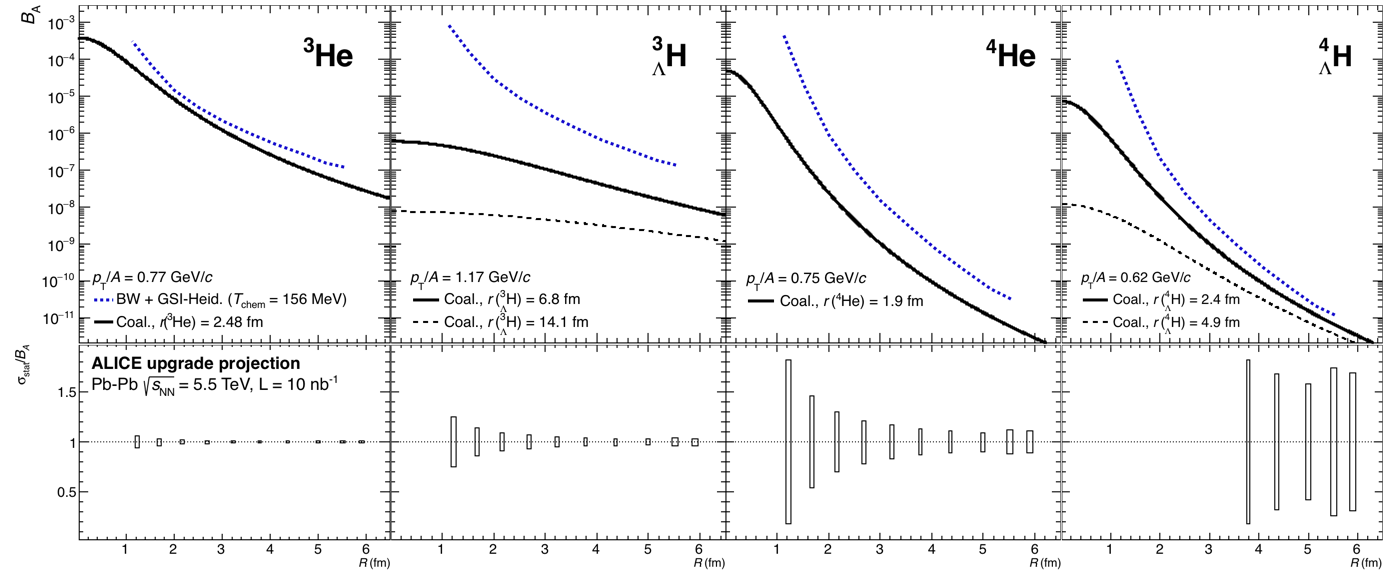
\includegraphics[width=\textwidth]{\main/lightflavour/figs/BAmodels_pseudoUnc.png}
\end{center}
\caption{
In the top panels the coalescence parameters for (hyper-)nuclei with $A = 3, 4$ are shown. Blue dashed lines are predictions from the thermal+blast wave model; black lines are coalescence predictions. For each (hyper-)nucleus, the rms radius is considered for the coalescence prediction as reported in the legend. Full details on the models are given in \cite{Bellini:2018epz}. The bottom panels show a projection of statistical significance in the discrimination between the two models that will be achieved with the Pb--Pb collisions integrated luminosity of 10 nb$^{-1}$.}
\label{fig:BAmodels}
\end{figure} 

\subsubsection{Light (anti-)(hyper-)nuclei production with the LHC Run 3 and 4}
The data-taking program with the upgraded ALICE detector after LS2 has a strong potential for measurements of nuclei, hypernuclei and the search for exotic states, because these studies require large event samples with a minimum-bias trigger, as well as high tracking precision for the separation of secondary vertices 
and charged-hadron (light nucleus) identification. The signal yields for the projected integrated luminosity of 10~nb$^{-1}$ were estimated for the 
(hyper-)nuclei (d,  \hethree, \hefour, \hyp, \hypfour, \hyphefour) and their antiparticles.
The theoretical production yields predicted by the the statistical hadronisation 
model~\cite{Andronic:2010qu} for central (0--10\%) Pb--Pb collisions 
%at \sqrtsNN = 2.76~TeV 
were considered. 
%This The predicted yields at \sqrtsNN = 5.5~TeV (the actual energy after LS2) are very close to those 
%at \sqrtsNN = 2.76~TeV~\cite{Andronic:2010qu}. 
The expected yield per unit of rapidity at mid-rapidity in the $\pt$\ range shown in the legend for d, \hethree\
and \hefour\ (and the corresponding anti-nuclei) are reported in left panel of Fig.~\ref{fig:yieldrun34}. 
%The predicted expected yields of the (hyper)nuclei in the 2-10\gmom\ $\pt$\ interval for $L_{\rm int} = 10$~nb$^{-1}$ are shown in the left panel of Fig.~\ref{fig:yieldrun34}. 
In the right panel, the expected significance of the of hyper-nuclei measurements in central Pb-Pb 
collisions in Run-3 and 4 as a function of the integrated luminosity is shown. The exploited decay channels to reconstruct the different hyper-nuclei are reported in the legend. 
The expected significance 
of \hyp, \hypfour\ and \hyphefour\ \textcolor{red}{is xxx, xx and xx}, respectively. The collected sample will enable 
very precise measurements of the production of \hyp\ and \antihyp\ and \textcolor{red}{first ever experimental observation} of \antihypfour\ and \antihehypfour.

\begin{figure}[ht]
\begin{center}
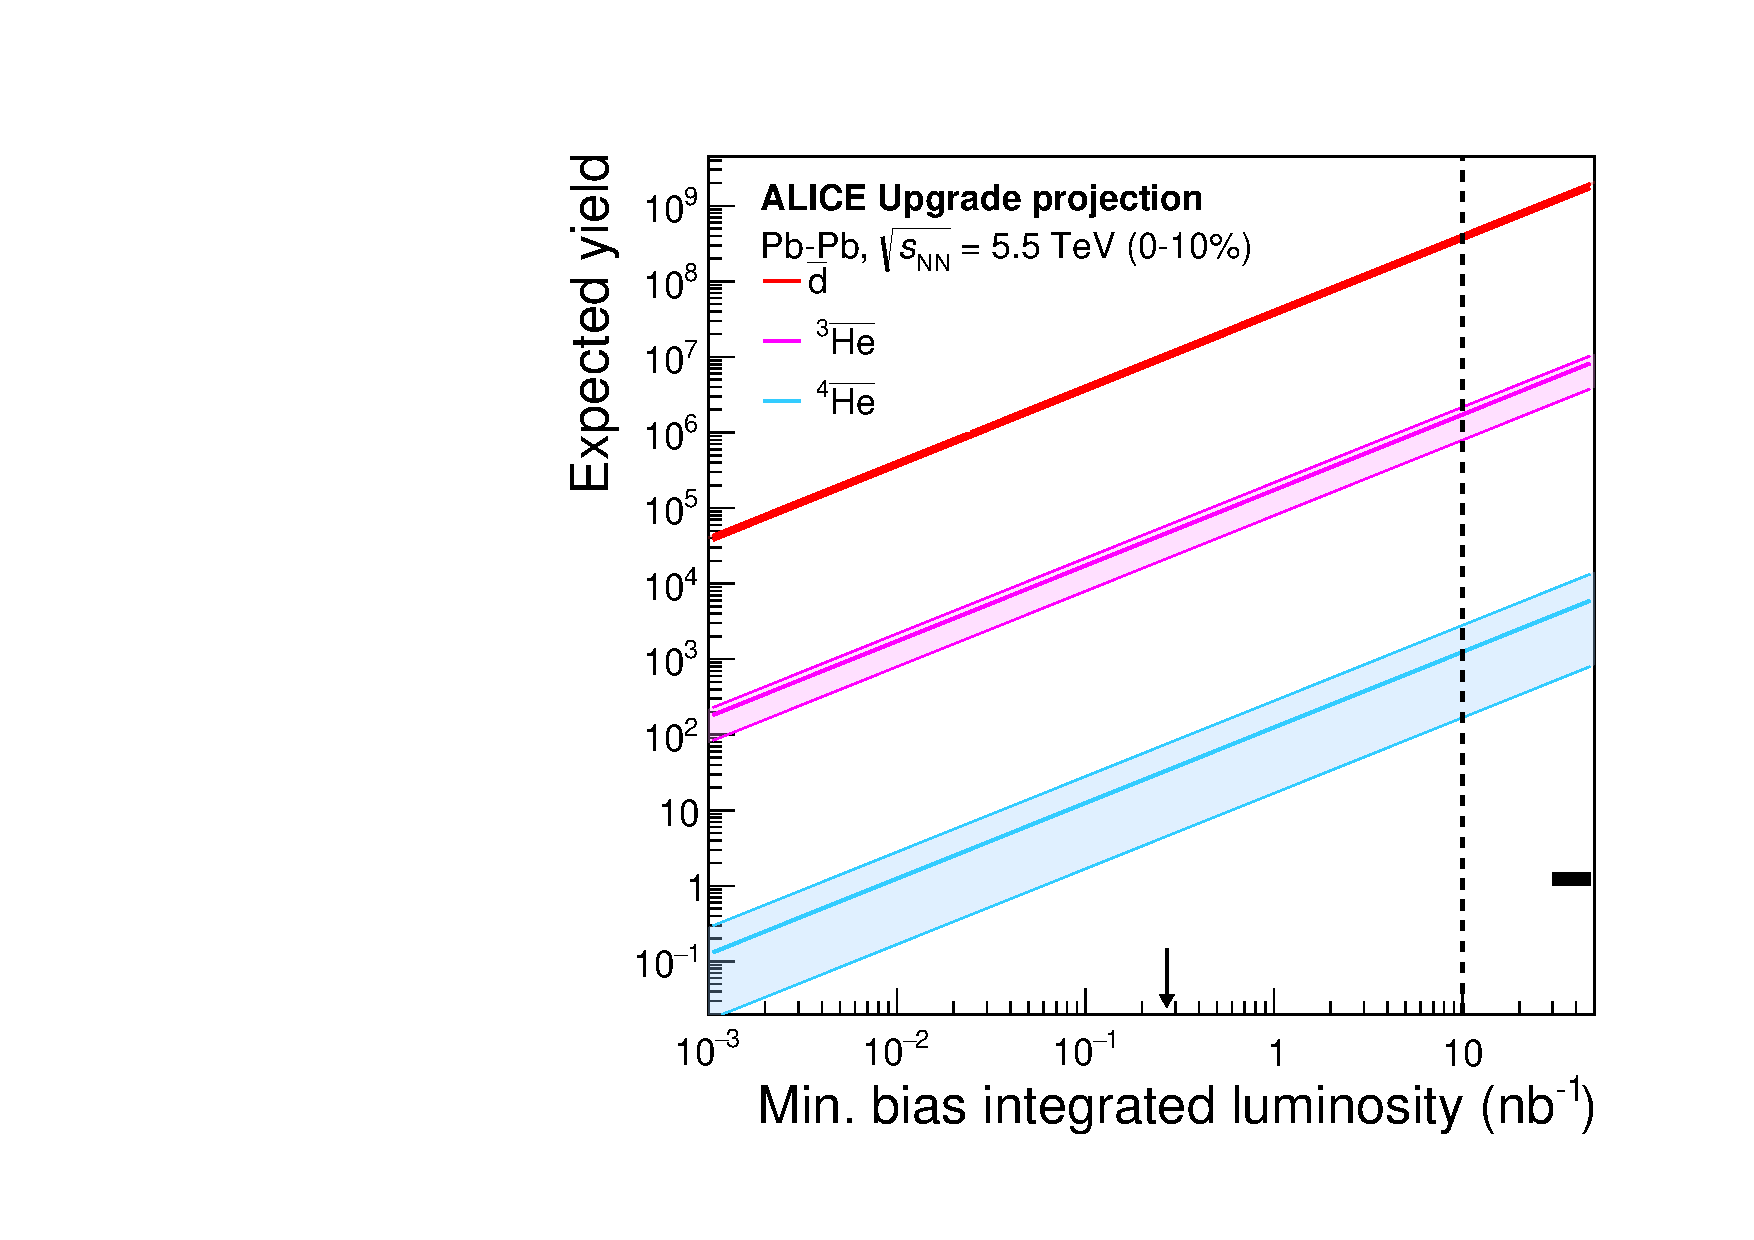
\includegraphics[width=0.45\textwidth]{\main/lightflavour/figs/nucleiYield.pdf}
%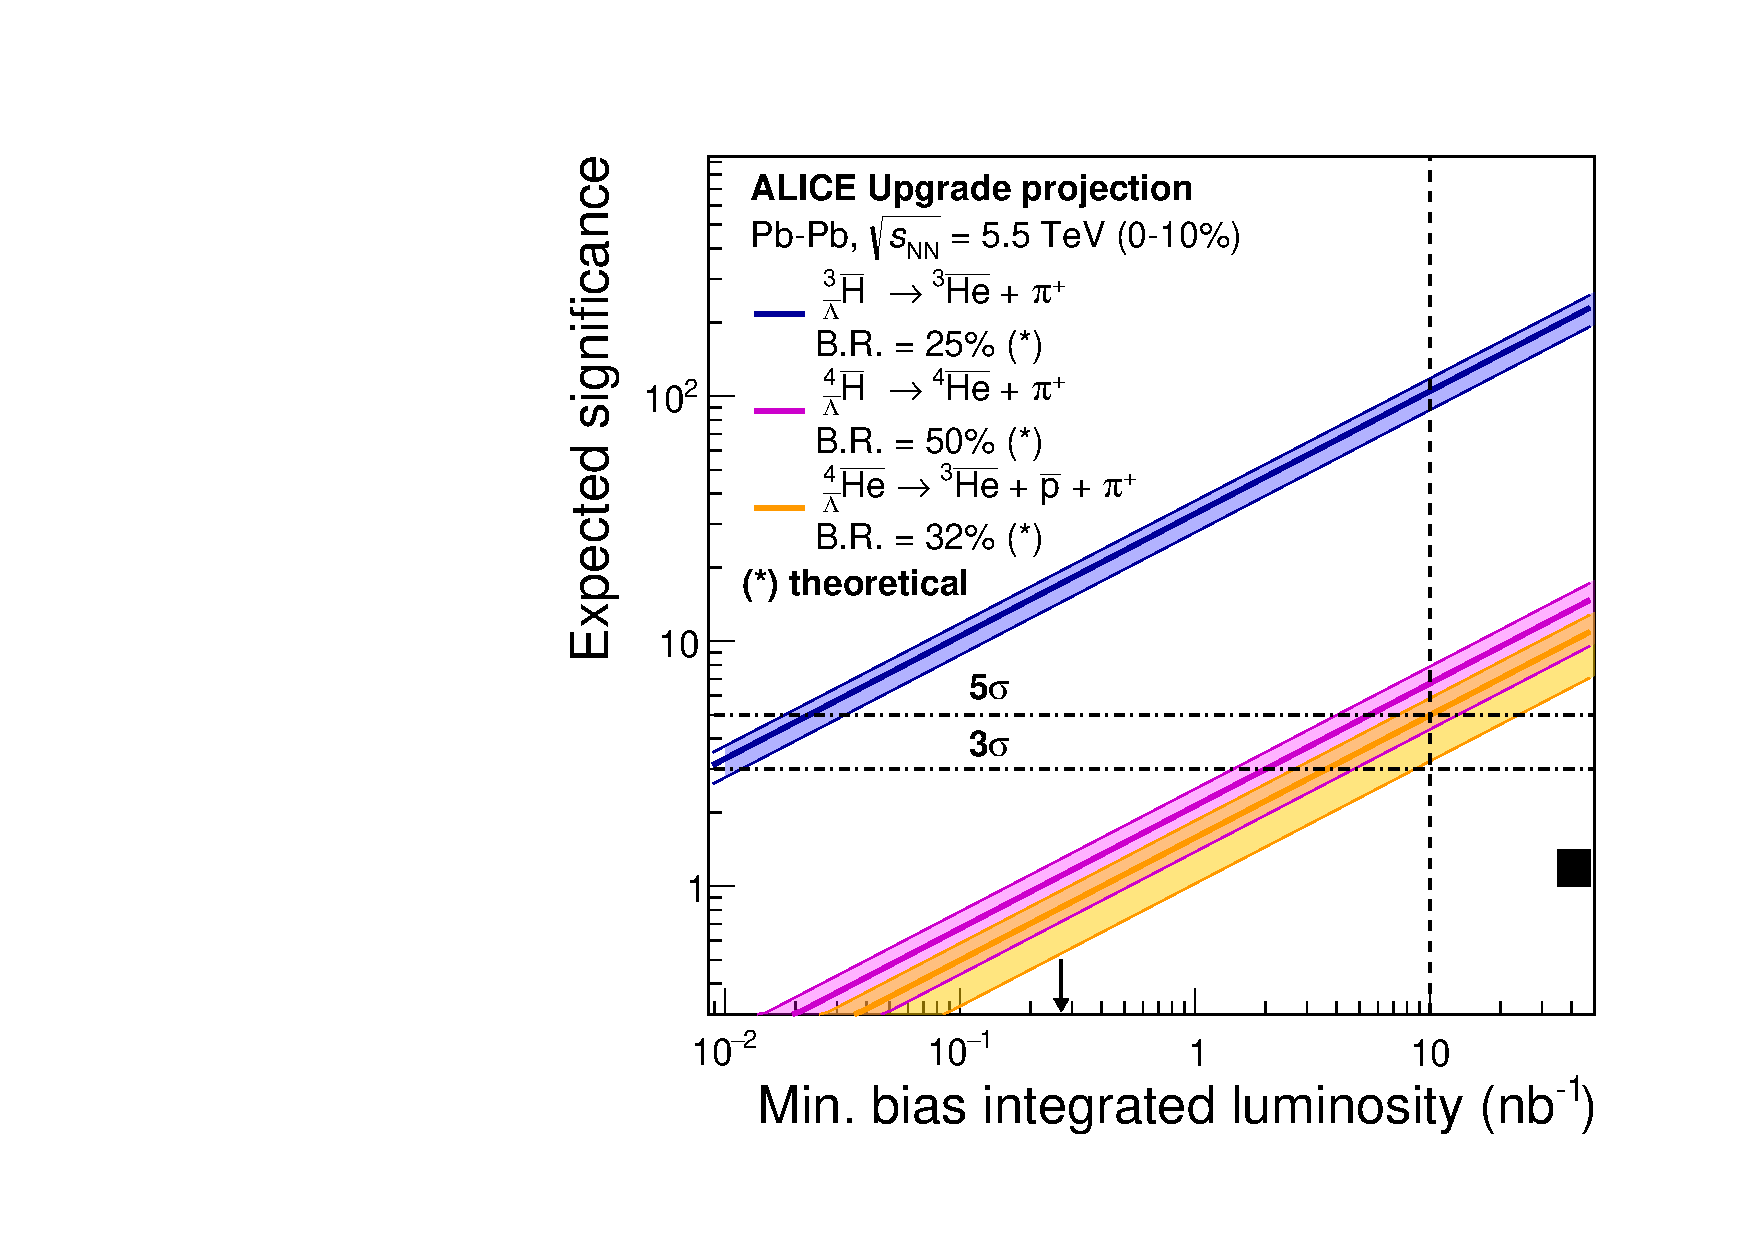
\includegraphics[width=0.32\textwidth]{\main/lightflavour/figs/hyperYield.pdf}
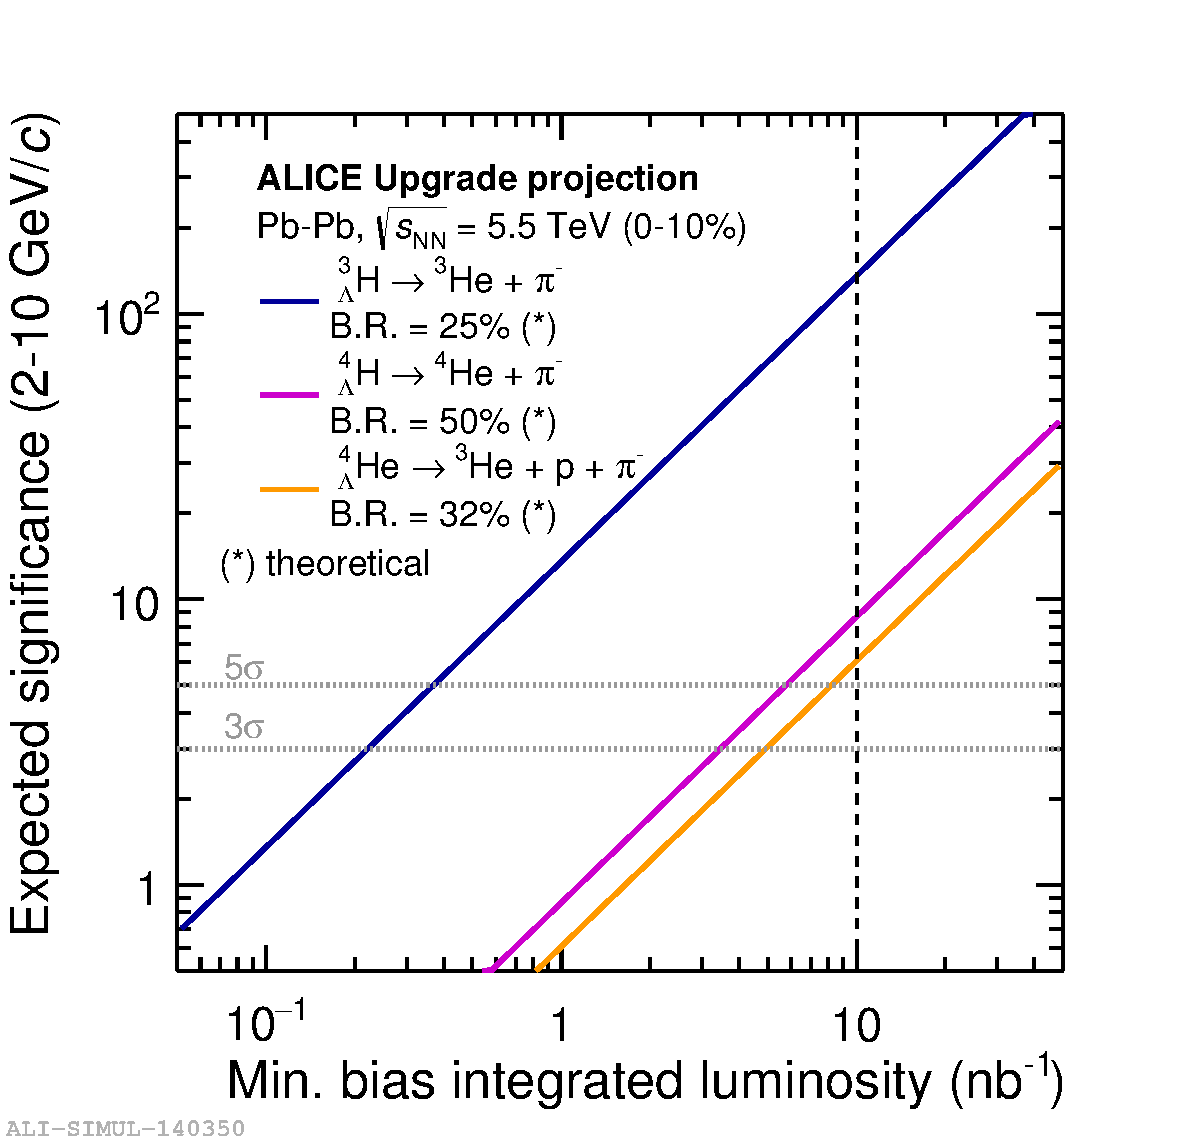
\includegraphics[width=0.45\textwidth]{\main/lightflavour/figs/hypernuclei_significance.pdf}
\end{center}
\caption{\textcolor{red}{To be updated.} Left: expected yield of (anti-)nuclei in 0--10$\%$ central Pb--Pb collisions as a function of the minimum bias luminosity. 
%Middle: expected yield of (anti-)(hyper-)nuclei as a function of the expected minimum bias luminosity. 
Right: Projected significance of hyper-nuclei measurements in central Pb-Pb collisions in Run-3 and 4 as a function of the integrated minimum bias luminosity. 
The vertical line represents the ALICE target.}
\label{fig:yieldrun34}
\end{figure}

\subsubsection{The hypertriton lifetime}
The hypertriton, \hyp, is a bound state of a proton, a neutron and a $\Lambda$.
The measured value of the $\Lambda$ separation energy, B$_{\Lambda}$ = 0.13 $\pm$ 0.05 (stat.) $\pm$ 0.04 (syst.) MeV \cite{davis20053}, led to the hypothesis that the lifetime of the hypertriton is equal or slightly below the free $\Lambda$ lifetime $\tau$($\Lambda$) = 263.2 $\pm$ 0.2 ps \cite{pdg:2017}.
Three different experimental techniques have been used to tackle this question: photographic emulsion, He bubble chambers and counter experiments. The average for the emulsion experiments is 203$^{+40}_{-31}$ ps \cite{agnello:2016}, for the He bubble chambers is 193$^{+15}_{-13}$ ps \cite{agnello:2016} and the combination of both visualizing techniques is 193$^{+14}_{-13}$ ps \cite{agnello:2016}. The counter techniques is used in heavy-ion experiments and the most recent results, 181 $^{+54}_{-39} \pm$ 33 ps and 142 $^{+24}_{-21} \pm$ 29 ps, have been obtained by the ALICE \cite{PhysLettB.754.360} and STAR \cite{PhysRevC.97.054909} experiments respectively. This techniques is that with the highest precision (14-16$\%$) at the moment and the weighted average of heavy-ion experiments results is 185$^{+28}_{-23}$ ps \cite{agnello:2016}.
However, the few existing theoretical calculations go in the direction of the hypothesis mentioned at the beginning of this section. The first approach to theoretical determination of $\tau$(\hyp) is due to Dalitz and Rayet and they obtained lifetime estimates in the range from 239.3-255.5 ps \cite{NuovCim.A46}. More recent calculations from Congleton \cite{jphysg.18.339} and Kamada \cite{Phys.Rev.C57} estimated a value of 232 ps and 256 ps, respectively.
The experimental results, previously reported and obtained with different techniques, and the theoretical calculations of $\tau$(\hyp) represents the "lifetime puzzle".

The future Run-3 and 4 data taking periods will be fundamental to solve the puzzle, since the projection is to reduce the statistical uncertainty between 1$\%$ and 0.5$\%$, with the expected integrated luminosity. 


\subsubsection{Exotica}
\textcolor{blue}{In preparation.}
%table 
\begin{table}[!h]
\begin{center}
\caption{\textcolor{blue}{Placeholder} Expected yields for exotic states for central Pb--Pb collisions (0--10\%) at $\sqrt{s_{\mathrm{NN}}} = 5.5$~TeV.} 
% From left to right: (hyper)nuclear species, production yield from the statistical hadronization model~\cite{Andronic:2010qu}, branching
% ratio (only for hypernuclei and exotica states), rapidity interval, and number of expected reconstructed particles for $L_{\rm int} = 10$~nb$^{-1}$~\cite{Abelevetal:2014dna} and reference for the estimation of the average acceptance-times-efficiency $\langle Acc. \times \epsilon\rangle$ for $p_\mathrm{{T}} > 0$.}

% \label{tab:yield}
% \begin{tabular}{lccccc}
% \hline
% State              & d$N$/d$y$                & B.R.   & $|y|<$ &  Yield                & Ref.\\
% \hline
% d (TPC)            & 5  $\times$10$^{-2}$  & -- &      0.5        &  3.1$\times$10$^{8}$ &\cite{Adam:2015vda}\\
% d (TPC+TOF)        & 5  $\times$10$^{-2}$  & -- &      0.5        &  1.4$\times$10$^{8}$ &\cite{Adam:2015vda}\\
% $^{3}$He (TOF)     & 3.5$\times$10$^{-4}$  & -- &      0.5        &  2.2$\times$10$^{6}$ &\cite{Adam:2015vda}\\
% $^{4}$He (TPC+TOF) & 7.0$\times$10$^{-7}$  & -- &      0.5        &  1.5$\times$10$^{3}$ &\cite{Adam:2015vda}\\
% $^{3}_{\Lambda}$H  & 1.0$\times$10$^{-4}$  & 0.25 &      1          &  4.4$\times$10$^{3}$ &\cite{Andronic:2010qu}\\
% $^{4}_{\Lambda}$H  & 2.0$\times$10$^{-7}$  & 0.50 &      1          &  1.1$\times$10$^{2}$ &\cite{Andronic:2010qu}\\
% $^{4}_{\Lambda}$He & 2.0$\times$10$^{-7}$  & 0.54 &      1          &  1.3$\times$10$^{2}$ &\cite{Andronic:2010qu}\\
% ${\Lambda}$n       & 3.0$\times$10$^{-2}$  & 0.35 &      1          &  2.9$\times$10$^{7}$ &\cite{Adam:2015nca}\\
% ${\Lambda\Lambda}$ & 5.0$\times$10$^{-3}$  & 0.064 &      1          &  1.9$\times$10$^{5}$ &\cite{Adam:2015nca}\\
% ${\Lambda\Lambda}$ & 5.0$\times$10$^{-3}$  & 0.41 &      1          &  1.2$\times$10$^{6}$ &\cite{Adam:2015nca}\\
% \hline
% \end{tabular}
\end{center}
\end{table}

